\documentclass[thesis.tex]{subfiles}
\begin{document}
The content of the previous chapter allow us to easily implement the equilibrated flux estimator, and present some (interesting) results.
We will analyze the unknown constants present in the error bounds using this implementation.
In particular we seek out to answer questions like:
\begin{itemize}
  \item How tight is the error bound given by the equilibrated flux estimator?
  \item What is the practical convergence rate of AFEM driven by the equilibrated flux estimator?
  \item How do the equilibrated flux estimator and classical estimator --- both optimal AFEM drivers --- compare to eachother?
  \end{itemize}


  \texttt{MATLAB} \cite{MATLAB:2015} is  used for the actual implementation. We 
  make extensive use of \texttt{iFEM}~\cite{chenifem}, a \texttt{MATLAB} framework for (adaptive) finite element methods. 
  All of the results are gathered for the \emph{linear} Lagrange finite element space $\VV(\T)$.
  We let \texttt{iFEM}  calculate the linear discrete solution $U$ for a given partition $\T$.
  The package ships with an implementation of the \emph{newest vertex bisection} refinement algorithm.
  This refinement method bisects marked triangles and ensures conformity as well as shape regularity of the resulting triangulation.
  We will first assess some classical (non-adaptive) finite element solutions.  After this, we will
  investigate the performance of the adaptive finite element method driven by the (lowest order) equilibrated flux estimator. The results
  will be compared to the classical residual estimator. The implementation solves $\vzet$ from \eqref{eq:systemzeta} and uses the element-wise estimator from Theorem~\ref{thm:zetaupper}.

  \section{Exact error}

  For meaningful results we ideally want to compare the error bounds from Theorem~\ref{thm:zetaupper} with the \emph{exact} 
  error $\enorm{u - U}_\O$. Given the exact $u$, we can directly use the \texttt{iFEM} package to calculate $\enorm{u - U}_{\O}$.
  This is, unfortunately, not possible in most situations. If one knows the exact solution $u$ of an interesting problem, then
  the right hand side $f$ of the associated Poisson problem is almost never constant, rendering our implementation useless. 
  On the other hand, the exact solution $u$ of an interesting problem with a constant rigtht hand side $f$ is almost never known.
  We have two ways to overcome this problem. 
  
  The first is to treat the $f$ as if it was piecewise constant. That is, 
  we approximate $\ip{\psi_a f - \nabla \psi_a \nabla U, q_k}_K$ by the edge-midpoint quadrature and ignore this approximation error. Similarly we simply replace the
  data oscillation term $\uanorm{f - \div \v{\zeta}}_K$  by its edge-midpoint quadrature. 
  Provided that $f$ is sufficiently smooth, the effects of these extra errors are of higher order $h$, and thus should be insignificant for small diameter.
  
  The other approach is to use a constant $f$, without knowing the exact solution $u$. We propose to approximate the true error $\enorm{u - U}_\O$ by replacing $u$ with another finite element solution $U_\star$  --- quite dazzling if one thinks about it.
  To make this work we let~$U_\star$ be a solution on a finer triangulation $\T_\star \geq \T$, such that
  every element in $\T_\star$ is at least \emph{one} bisection away from its corresponding element in $\T$. We have
  \[
    \enorm{u - U}_\O \leq \uaenorm{u - U_\star}_{\O} + \uaenorm{U - U_\star}_{\O},
  \]
  where we hope --- which is most likely the case if $u$ possesses some smoothness --- that 
  $\uanorm{u - U_\star}_{\O} \ll \uanorm{U - U_\star}_{\O}$. 
  A straightforward implementation of this approximation follows from noting that $U$ lies in the finite element spaces $\VV(\T_\star)$
  for refined triangulations $\T_\star \geq \T$.  \texttt{iFEM}  conveniently provides a function that calculates the
  coefficients of $U$ with respect to the linear basis of $\T_\star$.
  
  \section{Error estimators}
  In the numerical results, we will compare the real error $\enorm{u - U}_\O$ with various estimators.
  Ignore data oscillation terms, then for a reliable and efficient estimator $\eta$ one has
  \[
    C_{\text{eff}} \eta \leq \enorm{u - U}_{\O} \leq C_{\text{rel}} \eta.
  \]
  We\footnote{In literature, the efficiency index is often plotted as ${\eta \over \enorm{u - U_k}_\O}$. We chose the inverse definition, because
  this is in line with our placement of the efficiency constant in Theorem~\ref{thm:assumptions}.}
 will calculate the efficiency index  $C_{\text{eff}}$ of an estimator $\eta$ as ${\enorm{u - U_k}_\O \over \eta}$.
  The equilibrated flux estimator satisfies $C_{\text{rel}} = 1$. Therefore, one would like its effiency
  index to be close to one, as this shows tightness of the estimator. 
  In the residual case, we do not know the value of $C_{\text{rel}}$, and thus tightness of the estimator
  cannot be deduced from the efficiency index alone.

  The \texttt{iFEM} package provides an implementation of the standard residual estimator $\eta_\text{res}(U,K)$.
  We compare this estimator against the lowest order equilibrated flux estimator~${\eta_{\text{eq}}(U,K)}$ from Theorem~\ref{thm:zetaupper},  i.e. for $\vzet \in \RT_0(\T)$ the solution of \eqref{eq:systemzeta} and 
  \[
    \enorm{u - U}_{\O} \leq \sqrt{\sum_{K \in \T} \eta^2_{\text{eq}}(U, K)} \quad \text{with} \quad \eta^2_{\text{eq}}(U,K) :=  \left[ \uanorm{\vzet + \nabla U}_{K} + \frac{h_K}{\pi} \uanorm{ f - \div\v{\zeta}}_{K}\right]^2.
  \]
  \section{Uniform refinements}
  We start with classical finite element solutions: we let \texttt{iFEM} calculate
  the linear discrete solutions $(U_k)_{k \geq 0}$ for a sequence of uniformly bisected triangulations $(\T_k)_{k \geq 0}$, 
  i.e.~every triangle is bisected into four subtriangles.
  \begin{exmp}[Unit square]
    \label{ex:squaresin}
    Take the unit square domain $\O = (0,1)\times(0,1)$, with exact solution ${u(x,y) = \sin(2\pi x)\sin(2\pi y)}$. The corresponding Poisson problem is given by
  \begin{equation*}
    \begin{alignedat}{2}
      -\Delta u &= 8\pi^2\sin(2\pi x)\sin(2\pi y)  \quad &&\text {in } \Omega, \\
      u &= 0 \quad &&\text{on } \partial\O.
    \end{alignedat}
  \end{equation*}
\end{exmp}
The exact solution $u$ has four peaks and is very smooth. \texttt{iFEM} uses third order quadrature to approximate the integrals containing $f$.
  The produced discrete solutions $U_k$ are visualized in Figure~\ref{fig:squareuh}.
The images clearly illustrate some convergence of the FEM solution. 
As $u \in H^2(\O)$, we expect that $\enorm{u - U_k}_{\O} \lesssim h \abs{u}_{H^1(\O)}$. For uniform refinements this
latter is equivalent to $\enorm{u - U_k}_{\O} \lesssim N^{1/2} \abs{u}_{H^1(\O)}$, with $N$ the total number of vertices.
  \begin{figure}
    \centering
    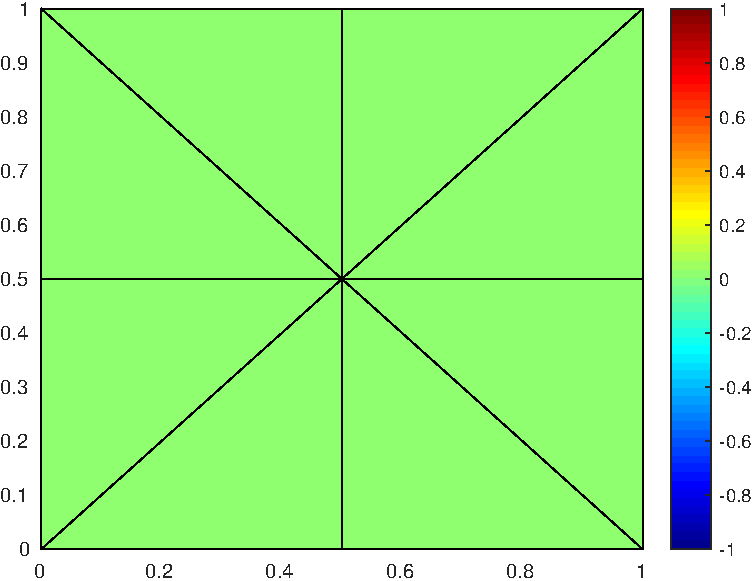
\includegraphics[width=.32\linewidth]{square_sin/mesh_uh_1.pdf}
    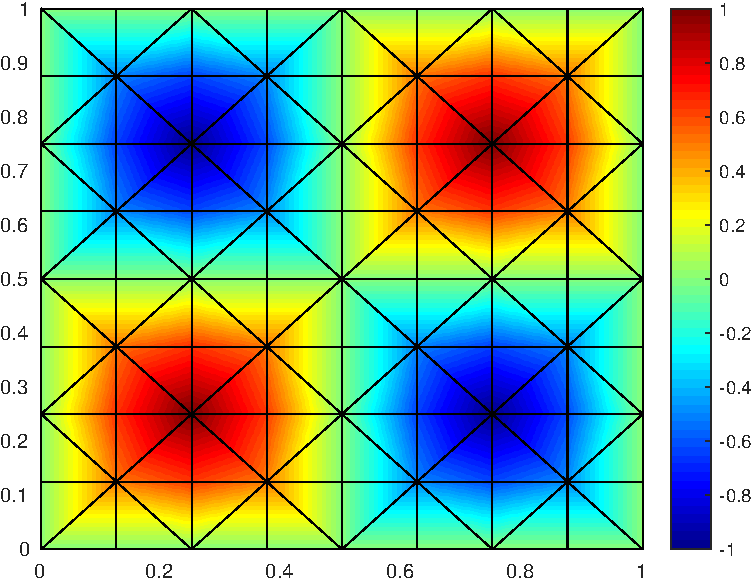
\includegraphics[width=.32\linewidth]{square_sin/mesh_uh_3.pdf}
    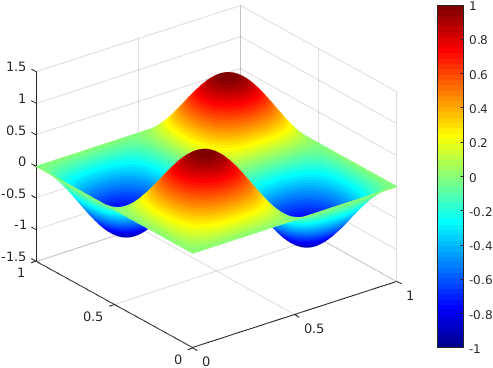
\includegraphics[width=.32\linewidth]{square_sin/result_uh_8.png}
    \caption{The finite element solutions $U_k$ for Example~\ref{ex:squaresin} with  uniformly bisected triangulations, from left to right we have diameters $h = 2^{-1}, 2^{-3}, 2^{-8}$.}
    \label{fig:squareuh}
\end{figure}

\begin{figure}
  \centering
  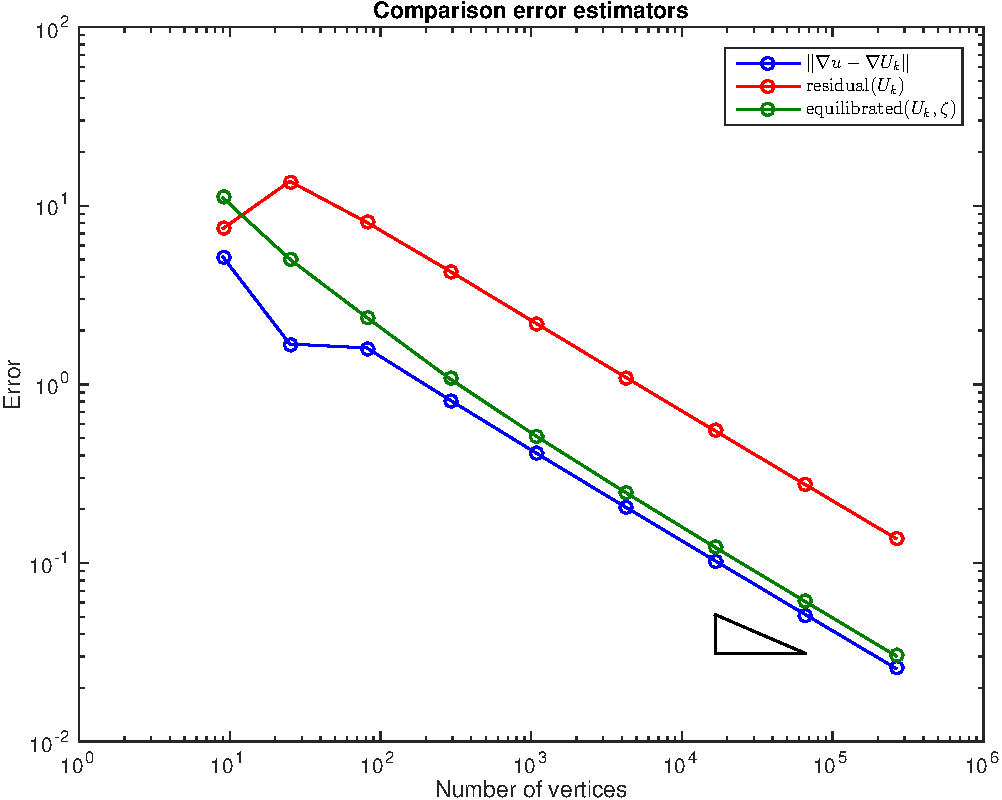
\includegraphics[height=.400\linewidth]{square_sin/norm_slope_9.pdf}
  \includegraphics[height=.400\linewidth]{square_sin/efficiency_9.pdf}
  \caption{Results for discrete solutions $U_k$ of the sinus  unit square (Example~\ref{ex:squaresin}) using a sequence of uniformly refined triangulations.  The left compares the exact error in the energy norm with the standard residual estimator and the equilibrated flux estimator.    The triangle has a slope of~$-1/2$. The right figure plots $\enorm{u - U_k} / \eta$; an estimation of the efficiency index.}
  \label{fig:squareerror}
\end{figure}

Results of the actual error (estimators) are given in Figure~\ref{fig:squareerror}.
The experimental convergence rate is in line with the theoretical convergence rate, as can see using the slope triangle.
The efficiency indices of $\eta_\text{eq}$ and $\eta_\text{res}$ differ greatly. The equilibrated flux estimator is about four times closer
to the real error than the residual estimator.
The efficiency index of the equilibrated flux estimator seems to increase, which could be explained by a reduction of quadrature errors for smaller diameters. 

We know the exact solution $u$ for this system, and thus we can empirically verify the claim that $\enorm{u - U_k}_{\O}$ is approximately  equal
to $\enorm{U_{k+i} - U_k}_{\O}$ for $i\geq 1$.
A comparison for  $i=1,2,3$ is given in Figure~\ref{fig:squareapprox}. The quality
of the error approximation increases with~$i$ as expected. 
\begin{figure}
  \centering
  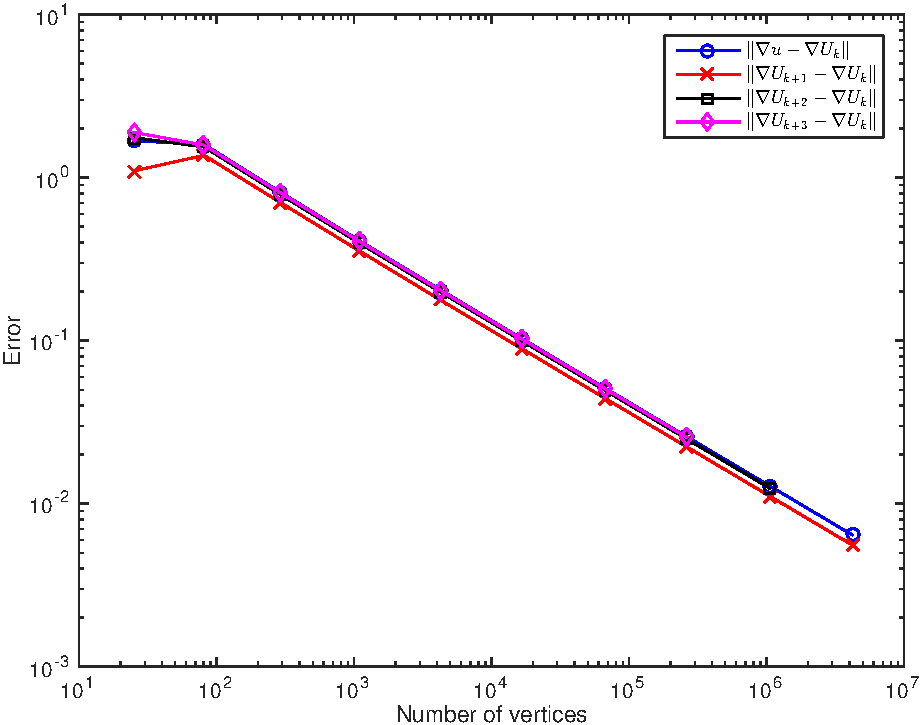
\includegraphics[width=.49\linewidth]{square_sin/approx_H1_10.pdf}
  \includegraphics[width=.49\linewidth]{square_sin/approx_H1_rel_10.pdf}
  \caption{ A comparison of the exact error $\enorm{u - U_k}_{\O}$ with the approximation $\enorm{U_{k+i} - U_k}_{\O}$ ($i=1,2,3$) for Example~\ref{ex:squaresin}. The left image plots all the norms, which results in a cluttered image as expected.
    The right image
  displays the relative terms, i.e.~$\enorm{U_{k+i} - U_k}_{\O} / \enorm{u - U_k}_{\O}$.}
  \label{fig:squareapprox}
\end{figure}


\begin{exmp}
  \label{ex:squareana}
Another Poisson problem for the unit square domain is given by 
\[
  u(x,y) = 2^{40}x^{10}(1-x)^{10}y^{10}(1-y)^{10}.
\]
This problem has homogeneous Dirichlet boundary conditions.
\end{exmp}
The corresponding right hand side $f$ is a high order polynomial; we let \texttt{MATLAB} derivate  it using symbolic calculations. The
solution $u$ has a peak of value $1$ centered around $(\frac{1}{2}, \frac{1}{2})$ and is again very smooth. In Figure~\ref{fig:squareana}
the efficiency indices are given, alongside the relative errors generated by $\enorm{U_{k+i} - U_k}_{\O}$ for this new problem. The 
initial triangulation~$\T_0$ is equal the one used in the previous problem.
The efficiency of the equilibrated flux estimator is less for this problem, which is most likely due to the large oscillation factor,
but it still outperforms the classical residual estimator. 

The behaviour of $\enorm{U_{k+i} - U_k}_\O$ is very similar to that of the previous problem; it appears to be a good estimation of
the exact error $\enorm{u - U_k}_{\O}$.
In the following problems we will treat this approximation as the `true error', since we no longer have a closed
form of the exact solution $u$.
For accuracy reasons we pick $i=3$, which should be good enough for a true error indicator.
We will write $U_{\star,k}$ for the discrete solution on $\T_{\star,k}$,
the triangulation found by uniformly refining every triangle in $\T_k$ three times.

\begin{figure}
  \centering
  \includegraphics[width=.48\linewidth]{square_ana/efficiency_9.pdf}
  \includegraphics[width=.50\linewidth]{square_ana/approx_H1_rel_10.pdf}
  \caption{Results for the square peak (Example~\ref{ex:squareana}). Left image compares the efficiency indices of the standard residual estimator with the equilibrated flux estimator. Right image
  shows the exact error approximation quality. }
  \label{fig:squareana}
\end{figure}

\begin{exmp}[Re-entrant corner]
  \label{ex:lshape}
  Here we consider the domain $\O = (-1,1)^2\setminus[-1,0]^2$, is also known as the L-shaped domain. 
  We will approximate the Poisson problem 
  \[
      -\Delta u= \1 \quad \text {in}\,\, \Omega, \quad\quad u = 0 \quad \text{on} \,\, \partial\O.
  \]
The solution $u$ of this problem has a singularity at the origin, so
that $u \not \in H^2(\O)$. 
\end{exmp}

We calculate  discrete solutions $U_k$ for uniform refinements. The 
exact solution~$u$ is uknown, and thus we will use $\uaenorm{U_{\star,k} - U_k}_\O$ as a true error indicator.
The results are given in Figure~\ref{fig:lshapeone}. The experimental
convergence of the FEM solution appears to be of order $h^{2/3}$.
The equilibrated flux estimator has a better efficiency index than the classical residual estimator.
There is a drop in terms of efficiency compared with the previous problems, because of the singularity $u$ has at the origin.
Interestingly, the efficiency of the equilibrated
estimator seems to decrease, whereas the efficiency of the standard estimator is somewhat increasing in $N$. 
This might be related to the approximation quality of $\uaenorm{U_{\star,k} - U_k}_{\O}$.

\begin{figure}
  \centering
  \includegraphics[height=.40\linewidth]{lshape_one/norm_slope_8.pdf}
  \includegraphics[height=.40\linewidth]{lshape_one/efficiency_8.pdf}
  \caption{Error estimators and their efficiency for the re-entrant corner domain (Example~\ref{ex:lshape}). The triangle has a slope of $-1/3$.}
  \label{fig:lshapeone}
\end{figure}

\begin{exmp}[Crack domain]
  \label{ex:crack}
  We solve $f = \1$ and $u = 0$ on $\partial \O$, on the crack domain
  \[
  \O=\{(x,y) \in \R^2 : |x|+|y|<1\}\setminus ([0,1] \times \set{0}).
  \]
The solution $u$ has a line singularity.
\end{exmp}
This domain is implemented by adding the vertex $(1,0)$ twice.  
The results are given in Figure~\ref{fig:crackone}.
The theoretical convergence rate on uniformly refined triangulations is of order $h^{1/2}$. This is even lower than the
rate from the previous example, because we now have an entire line singularity.
There is a drop in the efficiency index compared to the re-entrant corner; this could
be explained by the fact that $u$ is less regular. The overall behaviour of the efficiency is similar
to the previous example: the efficiency of the equilibrated flux estimator seems to decrease, 
while the efficiency of the residual estimator increases.
\begin{figure}
  \centering
  \includegraphics[height=.40\linewidth]{crack_one/norm_slope_8.pdf}
  \includegraphics[height=.40\linewidth]{crack_one/efficiency_8.pdf}
  \caption{Error estimators and their efficiency for the crack domain (Example~\ref{ex:crack}). The triangle has a slope of $-1/4$.}
  \label{fig:crackone}
\end{figure}

\section{Adaptive finite element method}
The convergence rates obtained for these last two examples is lower than rates found in the first
two (smooth) examples. This is a direct consequence of the singularities appearing in these last two examples.
These rates can be improved using the adaptive finite element method. The \texttt{iFEM} package contains
an implementation of newest vertex bisection refinement and D\"orfler marking, making it easy
to implement the adaptive method. We will restrict ourself to a constant right hand side $f$, because this
avoid the effects of data oscillation, and thus makes the total error indicator $\vartheta$ --- necessary for the AFEM optimality proof ---
equal to the estimator $\eta$. 

Recall that the equilibrated flux estimator $\eta_{\text{eq}}$ used here differs from the patch-wise estimator, 
$\uanorm{\v{\zeta_a} + \psi_a \nabla U}^2_{\w_a}$, used in the optimality AFEM proof.
Since these are closely related, it is reasonable to expect some sort of optimality from the above version as well 
(see the discussion in \S\ref{sec:remarks}). The advantage of the element-wise estimator $\eta_{\text{eq}}$ is that
we can mark elements instead of patches --- allowing us to use \texttt{iFEM} directly. 

The D\"orfler marking parameter $\theta$ used in AFEM must be small enough to ensure optimality
This D\"orfler upper bound is defined in terms of the efficiency constant
and the \emph{discrete} reliability constant, see Theorem \ref{thm:assumptions} and Lemma \ref{lem:dorfler}. Unfortunately,
we have no estimations of the discrete reliability constant. 
Earlier experiments, e.g. \cite{cascon2008}, show that $\theta = 1/2$ is often small enough.

The performance of AFEM driven by the equilibrated flux estimator 
is compared with AFEM driven by the classical estimator, and classical FEM using uniform refinements.
That is, we produce a sequence $(U_k, \T_k)_{k\geq0}$ of (A)FEM solutions for all of these three methods.
For each solution $U_k$ we measure its approximation error by $\uaenorm{U_{\star,k} - U_k}_\O$.


In Figure~\ref{fig:afem}, results are given for the crack domain and L-shaped domain using D\"orfler marking parameter $\theta = 1/2$.
One directly sees that the uniform convergence rate is improved 
by adaptivity --- as predicted by the theory.
 The AFEM solutions produced by the residual estimator and the equilibrated flux estimator
are of more or less the same quality.
This confirms our conjecture that AFEM driven by the (lower order) element-wise equilibrated flux estimator is also optimal.
It appears that eventually residual driven AFEM produces solutions with slightly
smaller approximation error. This might be related to the decreasing efficiency of the equilibrated flux  estimator,
cf.~Figures~\ref{fig:crackone} and \ref{fig:lshapeone}. 
\begin{figure}
  \centering
  \includegraphics[width=.49\linewidth]{lshape_one/afem.pdf}
  \includegraphics[width=.49\linewidth]{crack_one/afem.pdf}
  \caption{Comparison of (A)FEM methods on the L-shaped domain (left) and the crack domain (right). The three methods are
  compared by plotting the approximation error $\uaenorm{U_{\star,k} - U_K}_\O$ against the number of vertices. The adaptive methods
  used D\"orfler marking $\theta = 1/2$.}
  \label{fig:afem}
\end{figure}

\section{Mixed finite element solution}
Prager and Synge' theorem provided us with the following upper bound:
\[
  \enorm{u - U}_{\O}^2  \leq \norm{\nabla U - \vsig}^2_{\O} \quad \text{ for } \vsig \in H(\div; \O) \text{ s.t. } \div \v{\sigma} + f = 0
\]
The equilibration method constructs $\v{\zeta} \in \RT_p(\O)$ such that $-\v{\zeta}$ satisfies the equilibrium condition, and thus we find an
upper bound in terms of $\nabla U + \v{\zeta}$. As noted before, the best upper bound in the Raviart-Thomas space is found by minimizing
$\norm{\nabla U - \vsig}^2_{\O}$ over all fluxes $\vsig \in \RT_p(\O)$ that are in equilibrium. The mixed finite element method
provides the flux $\v{\sigma_{m}}$ that globally minimizes this norm. 
Since this method is too expensive for an estimator
calculation, the method of minimizing local problems was introduced. 
This makes it interesting to compare the performance of the equilibrated flux estimator with the mixed flux estimator
$\uanorm{\nabla U - \v{\sigma_m}}_\O$.

The \texttt{iFEM} package ships with an implementation of the lowest order mixed finite element solution. Figure~\ref{fig:effmixed} gives the efficiency
indices of the mixed- and equilibrated flux estimator for the example problems using uniform refinements. 
The mixed flux estimator has a higher efficiency index in all examples --- as one would expect. 
More surprising is the behaviour on the unit square problems. The efficiency coefficients of the equilibrated flux estimator
seem to converge to the efficiency index of the mixed flux estimator. This suggests that the penalty of applying
local instead of global minimization decreases for fine triangulations. For the L-shaped and crack domain we have different behaviour,
both the efficiency indices seem to decreases for fine triangulations. 
\begin{figure}
  \centering
  \includegraphics[width=.73\linewidth]{mixed/efficiency.pdf}
  \caption{
    Compares the efficiency index of the equilibrated flux estimator (dashed lines) against the mixed flux estimator (solid lines), for
  four different domains indicated by color and marker styles.}
  \label{fig:effmixed}
\end{figure}

The mixed flux estimator provides an element-wise error estimator by restricting the norm to an element, i.e.~$\eta^2_\text{mix}(U, K) := \uanorm{\nabla U - \v{\sigma_m}}^2_K$. 
We can use this estimator to drive AFEM. 
Figure~\ref{fig:afemmixed} compares the AFEM performance of the various methods on cracked domain with the smaller D\"orfler
parameter $\theta = 3/10$.  As before, all of the estimators produce discrete solutions of the same approximation quality. This
suggests that the earlier marking parameter of $1/2$ was already small enough for optimality.
\begin{figure}
  \centering
  \includegraphics[width=.73\linewidth]{mixed/afem.pdf}
  \caption{
    Approximation quality of various (A)FEM solutions for the cracked domain. The adaptive solutions are found using $\theta = 3/10$.
  }
  \label{fig:afemmixed}
\end{figure}
\section{Zienkiewicz-Zhu Error Estimator}
The theoretical and numerical results show the potency of the equilibrated flux estimator. Unfortunately, this estimator and many other promising
estimators are not often used in practice. This is mainly due to the implementational complexity and cost of such estimators.
Instead, engineers tend to use far easier estimators. One well-known example is the \emph{Zienkewicz-Zhu} estimator 
\cite{zienkiewicz1987simple, zienkiewicz1992superconvergent}. It is praised for its simplicity and cost effectiveness.

The general idea is based on \emph{gradient recovery}. That is, one smoothens the discrete gradient $\nabla U$ to obtain a
recovered gradient $G_\T U$ in the larger space $\left[\VV(\T)\right]^2$. Here
one hopes that $G_\T U$ provides a better approximation of the exact gradient $\nabla u$ than the discrete gradient $\nabla U$.
If this is the case, we would get $\nabla u - \nabla U \approx G_\T U - \nabla U$ and thus the latter provides
an error estimator.  
Various gradient recovery strategies are documented in the literature, for an overview see \cite{zienkiewicz1992superconvergent}. 

The initial gradient recovery estimator proposed by Zienkiewicz and Zhu in \cite{zienkiewicz1987simple} is based on
the orthogonal projection of $\nabla U$ into $\left[\VV(\T)\right]^2$. Write $G_\T^*U$ for the orthogonal
projector onto $\left[\VV(\T)\right]^2$, then $G_\T^*U$ is given as the solution of
\[
  \ip{G_\T^*U, \v{v} }_\O = \ip{\nabla U,\v{v}}_\O \quad \forall \v{v} \in \left[\VV(\T)\right]^2.
\]
A function $\v{v} \in \left[\VV(\T)\right]^2$ is determined by its values at the vertices $a \in \V$,
because we consider the linear finite element space. Rewrite the above equation using the hat functions $\psi_a$ as basis for $\VV(\T)$.
This reveals that the values of $G_\T^*U$ at vertices $a \in \V$  are the solution of 
\begin{equation}
  \label{eq:zzproject}
  \sum_{a \in \V} (G_\T^* U)(a) \ip{\psi_a, \psi_b}_\O = \ip{\nabla U, \psi_b}_{\O} = \sum_{K \subset \w_b} \frac{\vol(K)}{3} \nabla U|_K \quad \forall b \in \V.
\end{equation}
The second equality holds because $\nabla U$ is a piecewise constant vector.

Solving the above equation is as expensive as calculating the discrete solution $U$ itself. To
reduce this computational cost, Zienkiewcz and Zhu \cite{zienkiewicz1987simple} propose to approximate the
above integrals using trapezoidal quadrature rule, i.e.~$\int_K g \approx \frac{\vol(K)}{3} \sum_{a \in \V_K} g(a)$. 
The recovered gradient $G_\T U$ is the solution of \eqref{eq:zzproject}, with the integrals calculated by this quadrature.
All hat functions $\psi_b$ with $b\ne a$ vanish at vertex $a$, and therefore we obtain the remarkably simple expression
for $G_\T U$ at a vertex $a \in \V$:
\[
  (G_\T U)(a) = \sum_{K \subset \w_a} \frac{\vol(K)}{\vol(\w_a)} \nabla U|_K.
\]
In other words, the recovered gradient $G_\T U$ at a vertex $a \in \V$ is simply the weighted average of $\nabla U$ over
elements in the patch $\w_a$. Notice that $\nabla U$ is piecewise constant, whereas
the recovered gradient $G_\T U$ is a continuous piecewise linear function. The recovered gradient $G_\T U$ is 
therefore possibly a better approximation of $\nabla u$ --- especially near the discontinuities of $\nabla U$.

The Zienkiewicz-Zhu (ZZ) estimator for an element $K$ is given by ${\eta_\text{ZZ}(U, K) := \norm{G_\T U - \nabla U}_K}$. We will
not provide theoretical details about reliability and efficiency of this estimator
\cite{rodriguez1994some,zienkiewicz1992superconvergent}, but only consider
the experimental performance. The patch-wise nature of this ZZ estimator provides
some resemblance with the equilibrated flux estimator.
It is clearly interesting to compare this cheap and simple ZZ estimator with the equilibrated flux estimator.

An implementation of the ZZ estimator is straightforward using the framework provided by \texttt{iFEM}. 
Numerical results for the ZZ estimator are given in Figure~\ref{fig:ZZ}.
One image displays the efficiency index of the ZZ estimator for the various examples using uniform refinements.
The results are fascinating! The efficiency index of the ZZ estimator is close to $1$ for all examples previously
studied. Compare these results to the efficiency indices of the equilibrated- and mixed flux estimator in Figure~\ref{fig:effmixed}.
The ZZ estimator outperforms both these (relatively) expensive flux estimators. 
\begin{figure}
  \centering
  \includegraphics[height=.40\linewidth]{ZZ/efficiency.pdf}
  \includegraphics[height=.40\linewidth]{ZZ/afem.pdf}
  \caption{
    The left image compares the efficiency index of the ZZ estimator for various domains.
    The right figure shows the quality of three (A)FEM produced sequences for the cracked domain (Example~\ref{ex:crack}). The adaptive solutions are found using D\"orfler marking parameter $\theta = 1/2$.
  }
  \label{fig:ZZ}
\end{figure}

This high accuracy is closely
connected to the polynomial degree used in the FEM space $\VV(\T)$. That is, the accuracy
is expected to drop if one uses higher order polynomials in the FEM space \cite{bartels2002each}.
There are different gradient recovery methods which are also stable for higher order polynomials.

The ZZ estimator can be used to drive AFEM. The right image in Figure~\ref{fig:ZZ} compares this ZZ driven AFEM method
with the AFEM results produced by the equilibrated flux estimator. The results are (again) gathered for the cracked domain 
(Example~\ref{ex:crack}). Unsurprisingly we see that the ZZ driven AFEM solutions are of the same quality as the ones produced by the
equilibrated flux estimator. 


\section{Discussion}
The numerical results in this chapter support the promising theoretical claims about the equilibrated flux estimator.
The efficiency index of the equilibrated flux estimator behaves well for all of the examples studied:
the lowest efficiency index of $\approx 0.55$ was found for the crack domain.
The estimator therefore provides tight error bounds, since its reliability bound is constant-free. 

Precision of the equilibrated flux estimator seems to be related to the smoothness of the exact solution. Indeed, the efficiency
index of the estimator decreases when comparing examples \ref{ex:squaresin}-\ref{ex:crack}.
Since these examples are ordered on regularity of $u$, this suggests that a less smooth solution $u$ negatively
effects the efficiency index. The mixed flux estimator $\eta_{\text{mix}}$ also follows this pattern.

Out of the estimators reviewed, the standard residual estimator has the worst efficiency index of approximately between $0.2$ and $0.3$.
Surprisingly, the ZZ-estimator provided the highest quality with an efficiency index near one. Quality of this estimator, however, is expected
to deteriorate if one considers higher order finite element spaces.
The convergence rate of AFEM driven by the various estimators is similar, as expected.

All results were gathered for the linear FEM space using the zeroth order equilibrated flux estimator. 
Furthermore, we used the element-wise estimator instead of the patch-wise version that was used to prove optimality. 
The numerical AFEM results
seem to provide optimal convergence rates, and therefore numerically confirm our conjecture from \S\ref{sec:remarks} stating
that AFEM driven by the element-wise equilibrated flux estimator is also optimal.

Unfortunately, the current implementation is not capable of calculating higher order equilibrated flux estimators. This limitation
leaves open some important research aspects. The most important aspect being the $p$-robustness of the estimator.
Future research has to be conducted to determine the behaviour
 of the equilibrated flux estimator under a variation of the polynomial degree used in the FEM space. 
This latter aspect could play a crucial role in the development of an optimal $hp$-AFEM algorithm.
\end{document}
